\section{Modellierung}
Der Aufbau des Hochregallagers wurde in diverse Bereiche unterteilt. Die wichtigsten sind das Hochregal selbst, wie auch das Regalbediengerät. Weitere sind die entsprechenden Zustände/Ereignisse, die innerhalb des Hochregallagers auftreten können. 
%
\subsection{Einheiten}
Die Basiseinheit ist Milimeter. Es ist jedoch möglich mit anderen SI-Einheiten (m, dm oder cm) zu arbeiten.
%
\subsection{Hochregal}
Das gesamte Hochregallager, oder auch der Lagerort, wird durch ein einzelnes Objekt dargestellt. Dieses Objekt enthält alle benötigten Informationen und ist als Singleton implementiert. Das heisst, dass auf die Gassen, das Regal und die Lagerfächer direkt zugegriffen werden kann. Dies bietet eine komfortables Arbeiten bei der Simulation und soll auch eine einfache Implementierung der Visualisierung ermöglichen. Weiter bietet es den Vorteil, dass alle Informationen über die Elemente des Lagerortes immer verfügbar sind und abgefragt werden können. Mit GetInstance() und den entsprechenden Get-Methoden des jeweils untergeordeneten Objekts kann auf jedes einzelne Element des Lagerorts zugegriffen werden.
%
\subsection{Regalbediengerät}
Innerhalb der Gasse bewegt sich nur das Regalbediengerät. Die Klasse RackFeeder bildet dies ab. Im vorherigen Abschnitt wurde auf die zulässigen Bewegungen eingegangen. Die maximalen Beschleuigungen, Verzögerungen und die Geschwindigkeit sind innerhalb dieser Klasse als Standardwerte definiert. Bei Bedarf lassen sie sich überschreiben.\\
Das Regalbediengerät (RackFeeder) kann nicht beliebige Bewegungen auchführen. Die einzig gültigen Bewegungen sind durch ein vollständiges Objekt definiert, es sind nur drei Bewegungen zulässig: 
%
\begin{itemize}
  \item Bewegung in yz-Achse
  \item Bewegung in x-Achse (dies ist vorhanden, jedoch wird es nicht verwendet, da in der Realität die Operationen in der Vorzone von einem zusätzlichen System wahrgenommen werden)
  \item Bewegung in u-Achse (in das Regalfach hinein zum Be- und Entladen des Lagergütes)
\end{itemize}
%
Dies verhindert, dass der RackFeeder physikalisch unmögliche Bewegungen ausführen kann und stellt sicher, dass in jedem Zustand nur die darin gültigen Bewegungen ausgeführt werden können.
%
\subsection{Ereignisse}
Innerhalb des Systems wurden die Ereignisse (Events) in die Operationen Einlagern und Auslagern zerlegt. Die Verzweigungen sind in den nachfolgenden Abbildungen in gelb dargestellt. Der Startpunkt ist blau und entspricht dem Verhalten im Wartemodus. 
%
\begin{figure}[H]
\subfigure[Einlagern]{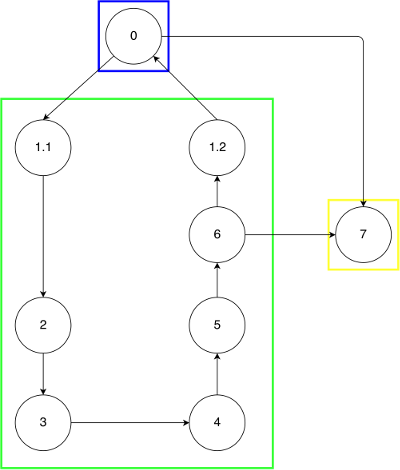
\includegraphics[width=0.49\textwidth]{images/einlagern.png}}\hfill
\subfigure[Auslagern]{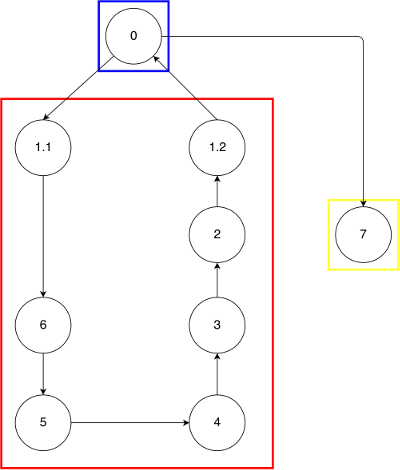
\includegraphics[width=0.49\textwidth]{images/auslagern.png}}
\caption{Verhalten}
\end{figure}
%
Die nachfolgende Tabelle zeigt auf der linken Seite die Einlagerung und auf der rechten Seite die Auslagerung.
%
\begin{table}[H]
  \begin{center}   
    \begin{tabular}{ccc|c|ccc}
		Eventnr.&	Koord.&	Zustand & & Eventnr.&	Koord.&	Zustand\\
		\hline
		1 &			0/0 &	empty & & 1 &			0/0 	&empty\\
		2 &			0/0 &	loaded & & 6 &			y/z 	&empty\\
		3 &			y/z &	loaded & & 5 &			x 		&empty\\
		4 &			x 	&	loaded & & 4 &			x 		&loaded\\
		5 	&		x 	&	empty & & 3 &			y/z 	&loaded\\
		6 	&		y/z &	empty & & 2 &			0/0 	&loaded\\
		1	&		0/0	&	empty & & 1	&		0/0		&empty\\
		7 &					&sleep& & 7 &					&sleep\\
    \end{tabular}
  \end{center}
\end{table}
%	
\subsection{Architektur}
Die Unterteilung der Anwendung erfolgte in einen Teil für die Modellierung, einen für die Simulation und einen für die Visualisierung. Diese Trennung macht die Anwendung in Bezug auf geänderte Lagerorte und Simulationensszenarien, oder auch für Optimierungen flexibel.
%
%
\begin{figure}[H]
  \begin{center}
    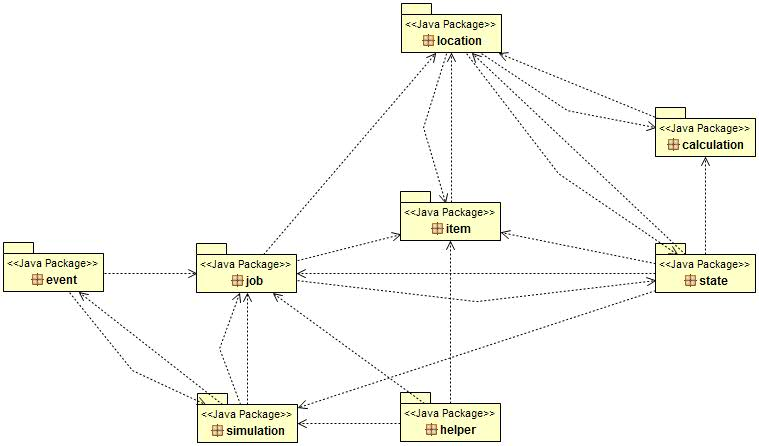
\includegraphics[width=0.6\textwidth]{images/package_diagramm.png}
    \caption{Package-Diagramm}
    \label{fig:packages}
  \end{center}
\end{figure}
%
\begin{figure}[H]
  \begin{center}
    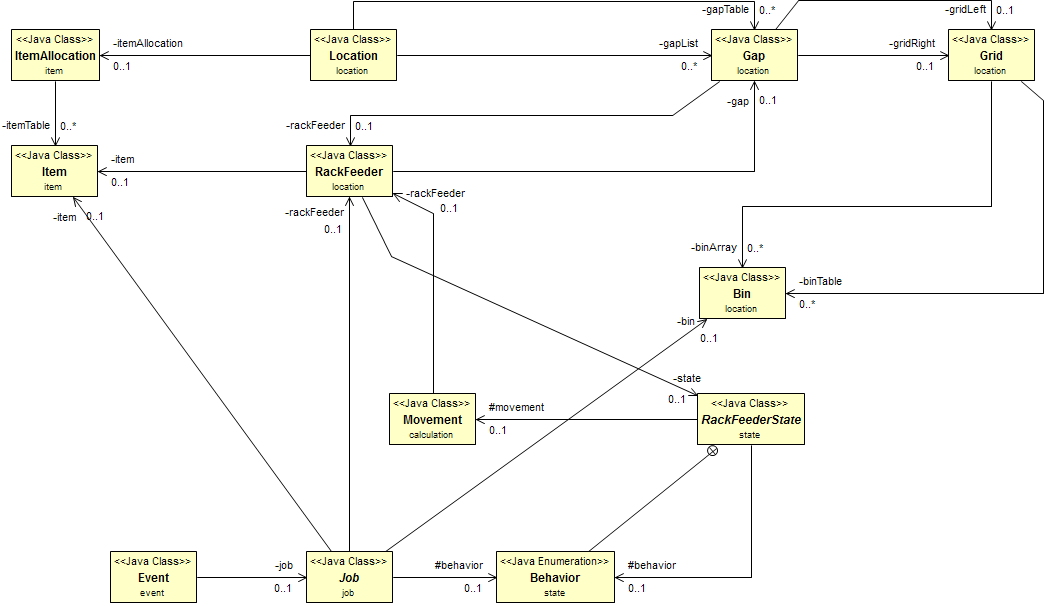
\includegraphics[width=0.6\textwidth]{images/class_diagramm.png}
    \caption{Class-Diagramm}
    \label{fig:class}
  \end{center}
\end{figure}
%
Die weiteren Diagramme befinden sich im Anhang.


%EOF
